\documentclass[11pt,a4paper]{article}
\usepackage[margin=1in]{geometry}
\usepackage{amsmath,amssymb}
\usepackage{booktabs}
\usepackage{graphicx}
\usepackage{float}
\usepackage[hidelinks]{hyperref}
\usepackage{titlesec}
\usepackage{placeins}
\usepackage{caption}
\captionsetup{font=small,labelfont=bf}
\setlength{\parskip}{0.4em}
\setlength{\parindent}{0pt}
\setlength{\textfloatsep}{8pt plus 2pt minus 2pt}
\setlength{\intextsep}{8pt plus 2pt minus 2pt}
\setlength{\abovecaptionskip}{4pt}
\setlength{\belowcaptionskip}{2pt}
\titleformat{\section}{\large\bfseries}{\thesection}{1em}{}
\titleformat{\subsection}{\normalsize\bfseries}{\thesubsection}{1em}{}

\title{\vspace{-3em}\textbf{Order Flow Imbalance and the Decay of Price Impact in CME Ether Futures}}
\author{Tony Li\thanks{Independent research conducted by the author; the views expressed are the author's own and not those of Imperial College London.}\\ \normalsize Imperial College London}
\date{May 2026}

\begin{document}
\maketitle

\begin{abstract}
\noindent We study Order Flow Imbalance (Cont, Kukanov, and Stoikov, 2014) on CME Ether futures over February 2021 to April 2026. On 25{,}546 out-of-sample dollar-volume bars (January 2024 to April 2026), an OLS regression of bar mid-quote change on contemporaneous OFI with Newey-West HAC standard errors yields $\hat{\beta} = +0.249$ ($t = 52.8$, $R^2 = 0.32$). Measured directly from the raw tick stream, the signal's forward impact rises over the first minutes, peaks near +21.6 bp at four hours, and reverses within a day. A vol-targeted strategy with a 10-minute clock cap, fitted jointly with six other parameters on the in-sample window, achieves out-of-sample Sharpe $+5.11$ at $-2.8\%$ maximum drawdown over 4{,}531 round-trip trades; fill prices reconstructed from the tick stream place realistic execution at $+3.5$ to $+3.8$, and rolling walk-forward re-selection reproduces the single-split figure at $+4.5$ to $+5.0$. The Hansen (2005) test for superior predictive ability (SPA) over the 1{,}920-configuration joint search space gives $p < 0.001$; the Deflated Sharpe Ratio (Bailey and Lopez de Prado, 2014) on the same trial set gives $P(\mathrm{SR}>0) = 0.958$. A direction-shuffled placebo that preserves entry times, exit times, and the long/short count returns mean Sharpe $-0.37$ over 200 seeds (none reach the strategy's out-of-sample Sharpe). Under a square-root impact model (Almgren and Chriss, 2000), Sharpe remains above $2.0$ up to \$10M of deployed capital under the base average-daily-volume assumption.
\end{abstract}

\section{Introduction}

Order Flow Imbalance (OFI), introduced by Cont, Kukanov, and Stoikov (2014), aggregates best-bid and best-offer quote arrivals into a signed measure of top-of-book pressure. The construction builds on the information-asymmetry mechanism of Hasbrouck (1991) and the flow-toxicity work of Easley, Lopez de Prado, and O'Hara (2012); the associated price-impact theory is reviewed in Bouchaud, Farmer, and Lillo (2009). On liquid US equities, contemporaneous OFI explains roughly two-thirds of bar-level mid-quote variation. The cryptocurrency evidence is thinner: Silantyev (2019) finds trade-flow imbalance dominates short-horizon prices on BitMEX XBT/USD, and Bieganowski and Ślepaczuk (2026) report OFI as the top SHAP feature in CatBoost ensembles on Binance Futures perpetuals. CME's Ether contract sits between these regimes: a regulated venue with thinner top-of-book depth than the equity tape and a higher tick-relative spread than either. The OFI literature has not addressed it directly; the closest crypto context is Makarov and Schoar (2020) on cross-venue arbitrage and Aleti and Mizrach (2021) on Bitcoin spot-futures integration.

This paper estimates the contemporaneous OFI signal-impact on CME ETH futures from February 2021 to April 2026 and asks whether the relationship is exploitable out-of-sample net of a 1-tick-per-side adverse-selection cost. The construction is the level-1 (best bid / best offer) form of Cont, Kukanov, and Stoikov on dollar-volume bars built from TBBO (trade-sampled top-of-book) events (Lopez de Prado, 2018). Forward signal-impact is characterised at sub-bar to 24-hour horizons; the bar regression alone cannot resolve the decay structure that determines holding-period choice.

\section{Data}

The panel consists of CME-cleared TBBO data for the front-month ETH futures contract, covering February 2021 through April 2026. After roll handling and contract stitching, the strategy operates on the front-month book.

Bars are constructed in dollar volume, with the threshold calibrated so that a median in-sample trading day produces about ten bars, and that threshold is held fixed when bars are constructed for the out-of-sample period.

For each bar the following quantities are computed:
\begin{itemize}
    \item \texttt{ofi}: signed level-1 (best bid / best offer) order flow imbalance, following the construction of Cont, Kukanov, and Stoikov (2014). For each TBBO update $i$, let $p^B_i, p^A_i$ denote the best-bid and best-ask quotes and $q^B_i, q^A_i$ their sizes. The per-event OFI contribution is $e_i = e^B_i + e^A_i$, where
    \begin{align*}
    e^B_i &=
    \begin{cases}
        +q^B_i              & \text{if } p^B_i > p^B_{i-1}  \\
        -q^B_{i-1}          & \text{if } p^B_i < p^B_{i-1}  \\
        q^B_i - q^B_{i-1}   & \text{if } p^B_i = p^B_{i-1}
    \end{cases},
    \qquad
    e^A_i =
    \begin{cases}
        -q^A_i              & \text{if } p^A_i < p^A_{i-1}  \\
        +q^A_{i-1}          & \text{if } p^A_i > p^A_{i-1}  \\
        -(q^A_i - q^A_{i-1})& \text{if } p^A_i = p^A_{i-1}.
    \end{cases}
    \end{align*}
    A best-bid improvement adds its new size as positive flow; a best-bid drop subtracts the displaced prior size; a same-price size change contributes the signed change. The ask side is symmetric with reversed sign. The bar OFI is the unnormalised sum over all events in the bar, $O_t = \sum_{i \in \text{bar } t} e_i$, with no normalisation by bar duration, depth, or volume. Only level-1 quantities enter the construction; the TBBO data source carries the touch and trades but not deeper book levels.
    \item \texttt{mid\_close}: the mid quote $(p^B + p^A)/2$ at the bar boundary.
    \item \texttt{d\_mid}: the change in mid quote since the previous bar.
\end{itemize}

\section{Signal-impact regression}
\label{sec:impact}

Following Cont, Kukanov, and Stoikov (2014) and Silantyev (2019), bar mid-quote change is regressed on contemporaneous and one-bar lagged OFI:
\begin{equation}
\Delta p_t = \alpha + \beta_0 \, O_t + \beta_1 \, O_{t-1} + \varepsilon_t,
\end{equation}
where $\Delta p_t = m_t - m_{t-1}$ is the change in mid-quote between bar boundaries and $O_t$ is the bar OFI. Standard errors are Newey-West HAC (Newey and West, 1987) with five lags. Table~\ref{tab:impact} reports the estimates on the full panel, the 2021-02 to 2023-12 in-sample (IS) window, and the 2024-01 to 2026-04 out-of-sample (OOS) window.

\begin{table}[H]
\centering
\small
\begin{tabular}{lrrrrrr}
\toprule
Window & $n$ (bars) & $\hat\beta_0$ & HAC $t(\beta_0)$ & $\hat\beta_1$ & HAC $t(\beta_1)$ & $R^2$ \\
\midrule
Full sample          & 37{,}890 & $+0.271$ & $+67.8$ & $-0.028$ & $-13.5$ & 0.31 \\
In-sample 2021--23   & 12{,}344 & $+0.300$ & $+44.9$ & $-0.025$ & $-7.0$  & 0.31 \\
Out-of-sample 2024--26 & 25{,}546 & $+0.249$ & $+52.8$ & $-0.030$ & $-12.2$ & 0.32 \\
\bottomrule
\end{tabular}
\caption{OLS, Newey-West HAC (five lags). $p < 10^{-6}$ on both coefficients in every window.}
\label{tab:impact}
\end{table}

\begin{figure}[H]
\centering
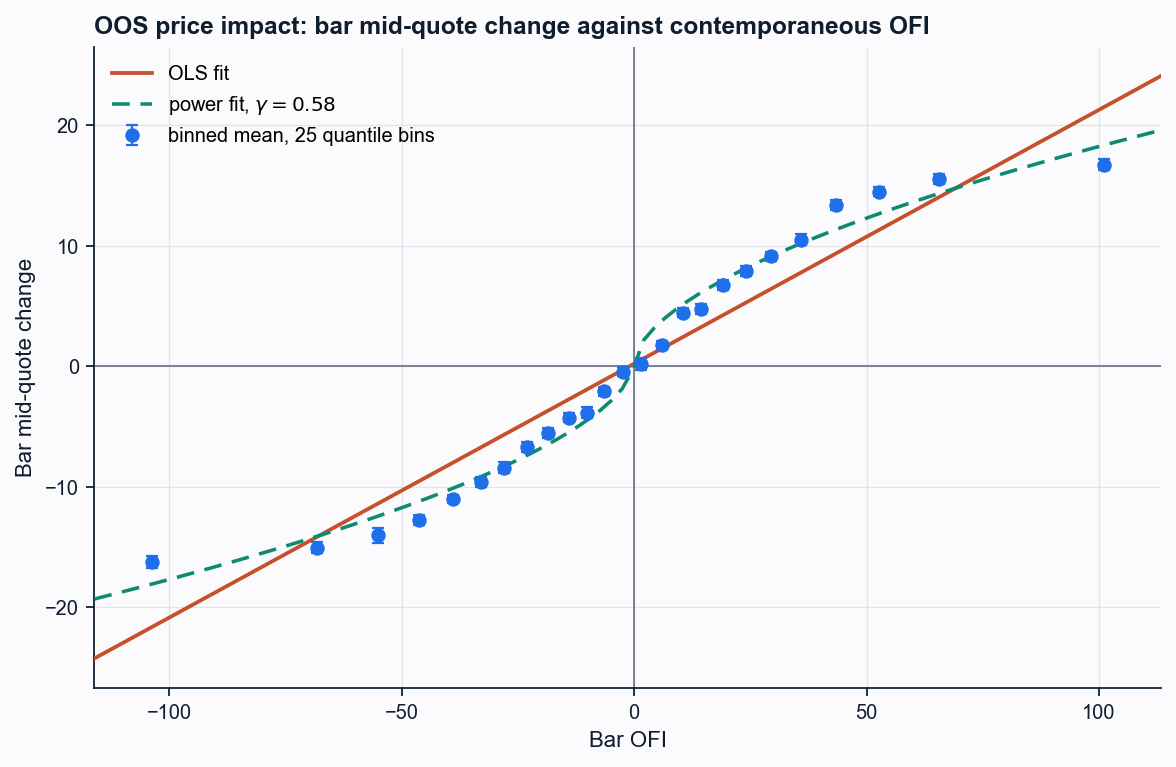
\includegraphics[width=0.82\textwidth]{fig5_impact.png}
\caption{Out-of-sample bar mid-quote change against contemporaneous OFI, 25 quantile bins with $\pm1$ standard error and the OLS fit. The relationship is close to linear; full estimates are in Table~\ref{tab:impact}.}
\label{fig:impact}
\end{figure}

Both subsamples reject $\beta_0 = 0$ at $p < 10^{-6}$. The IS $R^2$ of $0.31$ and OOS $R^2$ of $0.32$ match to within rounding, and the slope coefficient moves from $+0.300$ in-sample to $+0.249$ out-of-sample. Both $R^2$ figures are below the two-thirds level of Cont et al.\ (2014) for liquid US equities; CME Ether futures have lower depth and a higher tick-relative spread.

The OOS regression has a positive contemporaneous term $\beta_0 = +0.249$ (Figure~\ref{fig:impact}) and a negative one-bar-lagged term $\beta_1 = -0.030$, with the lag-1 reversion approximately $12\%$ of the contemporaneous impact. The regression is identified at bar resolution (mean OOS bar duration ${\approx} 47$ minutes); Section~\ref{sec:decay} characterises the signal's forward impact at sub-bar to 24-hour horizons directly.

\subsection{Signal decay profile}
\label{sec:decay}

The bar regression cannot resolve signal decay at sub-bar horizons. Forward impact is measured directly at 21 horizons from 30 seconds to 24 hours: for each of the 4{,}531 OOS entries, the mid-quote at the entry timestamp and at each horizon is taken from the raw TBBO, and the cumulative return is signed by entry direction. Measurements where the matched BBO at the target time is more than 120 seconds stale (e.g.\ past the daily 5--6 pm ET session break) are dropped, so the sample falls with horizon (Table~\ref{tab:decay}). A sign-randomised placebo at the same timestamps, averaged over 50 seeds, stays within $\pm 1.1$ bp of zero at every horizon and its $95\%$ band always covers zero; the OFI-direction curve is not market drift. Standard errors and confidence intervals are from a block bootstrap over trading days (2{,}000 resamples): the forward windows of nearby entries overlap, so a cross-sectional standard error understates uncertainty at long horizons. A non-overlapping subsample, keeping entries at least one horizon apart, is reported as a cross-check.

\begin{table}[H]
\centering
\small
\begin{tabular}{rrrrr}
\toprule
Horizon & Signed return (bp) & Block-bootstrap $t$ & $95\%$ CI (bp) & $n$ \\
\midrule
$0.5$ min  & $+3.19$  & $14.2$ & $[+2.8,\ +3.7]$   & $4{,}459$ \\
$1$ min    & $+5.92$  & $17.0$ & $[+5.3,\ +6.7]$   & $4{,}529$ \\
$2$ min    & $+8.50$  & $16.3$ & $[+7.5,\ +9.5]$   & $4{,}529$ \\
$10$ min   & $+10.16$ & $10.7$ & $[+8.3,\ +12.1]$  & $4{,}278$ \\
$30$ min   & $+12.83$ & $8.1$  & $[+9.8,\ +16.0]$  & $4{,}222$ \\
$1$ hour   & $+15.13$ & $6.5$  & $[+10.6,\ +19.7]$ & $4{,}091$ \\
$2$ hours  & $+16.89$ & $5.2$  & $[+10.5,\ +23.4]$ & $3{,}792$ \\
$4$ hours  & $+21.63$ & $4.7$  & $[+12.4,\ +30.6]$ & $3{,}660$ \\
$8$ hours  & $+6.22$  & $0.9$  & $[-7.3,\ +19.4]$  & $3{,}126$ \\
$12$ hours & $+5.94$  & $0.8$  & $[-8.7,\ +20.3]$  & $3{,}168$ \\
$24$ hours & $-9.42$  & $-0.8$ & $[-32.8,\ +14.6]$ & $2{,}917$ \\
\bottomrule
\end{tabular}
\caption{Mean forward signed return at fixed horizons after OOS signal entry. The $t$-statistic and $95\%$ interval are from a by-day block bootstrap (2{,}000 resamples), which keeps each day's overlapping forward windows together. A non-overlapping subsample (entries at least one horizon apart) gives $t = 3.8$ at the four-hour peak.}
\label{tab:decay}
\end{table}

\begin{figure}[H]
\centering
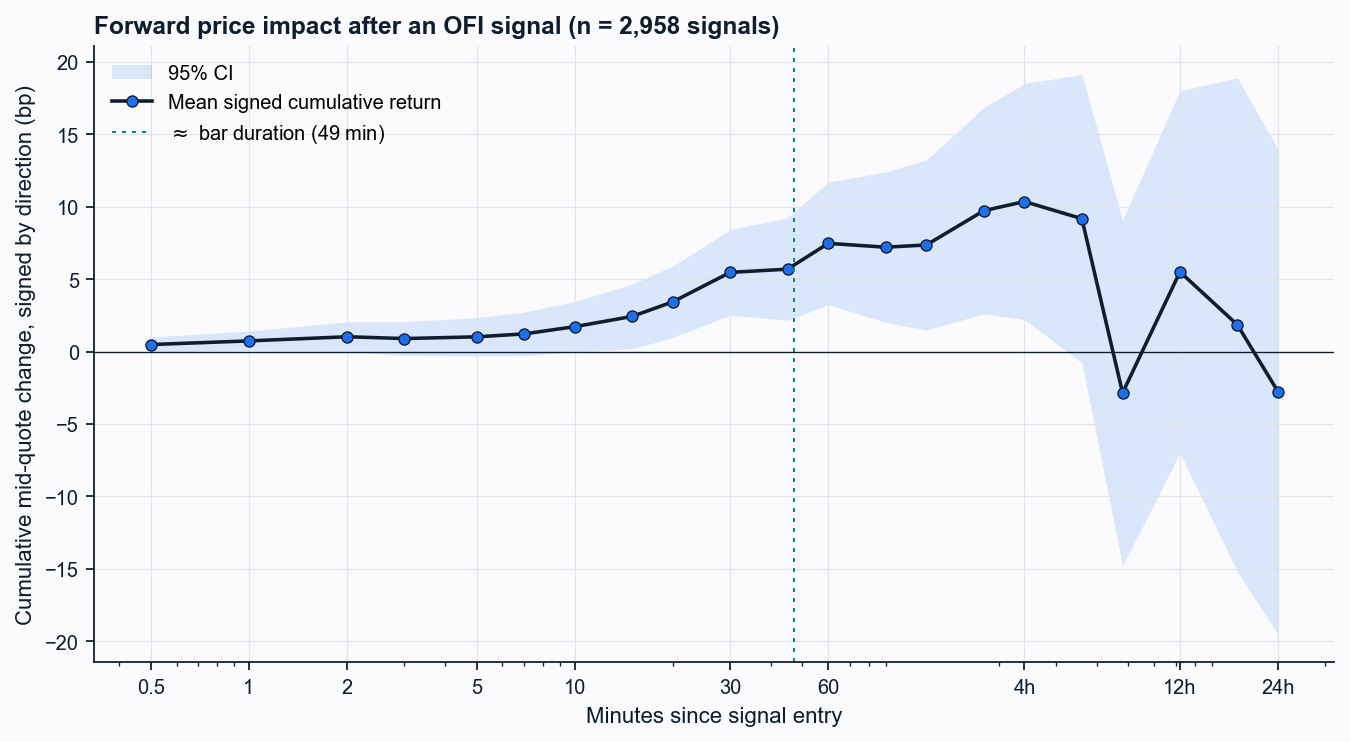
\includegraphics[width=0.92\textwidth]{fig4_decay.png}
\caption{Signed forward return after signal entry, OOS. Peak +21.6 bp at 4 hours; crosses zero by 24 hours.}
\label{fig:decay}
\end{figure}

The forward impact rises rapidly over the first two minutes, slows through the bar horizon, peaks at $+21.6$ bp at four hours, and decays to $-9.4$ bp at $24$ hours. The four-hour peak remains significant after the overlap correction (block-bootstrap $t = 4.7$, $95\%$ CI $[+12.4,\ +30.6]$ bp; non-overlapping subsample $t = 3.8$); the cross-sectional statistic overstates it, and beyond eight hours the signed return is not distinguishable from zero. The bar regression's $\beta_1$ reversion is small relative to the longer-horizon dynamics in Figure~\ref{fig:decay}. The 10-minute cap exits at about $10$ bp realised. The cap value comes from IS optimisation (Section~\ref{sec:params}) and is a Sharpe-maximising vol-control parameter; the decay profile characterises the signal independently of that choice.

\section{Strategy}

The trading signal is the rolling $z$-score of cumulative OFI over $K=5$ bars,
\begin{equation}
z_t = \frac{C_t - \mu_t}{\sigma_t}, \quad C_t = \sum_{s=t-K+1}^{t} O_s,
\end{equation}
with $\mu_t$ and $\sigma_t$ the trailing mean and standard deviation of $C$ over a 200-bar window shifted by one bar. A long opens at $z_t \geq 1$, a short at $z_t \leq -1$; exit on a zero-cross, after $H=3$ bars, on a contract roll, or on a 10-minute wall-clock cap, whichever comes first. The cap is a risk-shaping device: removing it lifts annualised vol from $6.9\%$ to $12.6\%$ and the drawdown from $-2.8\%$ to $-9.0\%$ (Table~\ref{tab:summary}). The 10-minute value comes from the IS sweep below. Decisions made on bar $t$'s close affect PnL only from bar $t+1$ onwards. The clock cap fires at wall-clock times that do not align with bar timestamps; the cap-fire bar's PnL is apportioned linearly by elapsed fraction.

Size is volatility-targeted at $15\%$ annualised on \$1M notional,
\begin{equation}
n_t = \max\!\left(1,\; \frac{0.15 \times 1{,}000{,}000}{\mathrm{mult}_{\mathrm{ETH}} \cdot \mathrm{mid}_t \cdot \hat{\sigma}_{\mathrm{ann},t}} \right),
\end{equation}
with $\hat{\sigma}_{\mathrm{ann},t}$ the 200-bar rolling annualised vol of bar returns. The 1-contract floor binds only in low-vol regimes. Execution is assumed to be that of a colocated proprietary participant, with intra-bar fills at the touch and no rebate capture; the headline Sharpe is computed at a 1-tick adverse-selection cost (\$2.50/contract, $\approx 0.16$ bp at typical front-month prices), and Table~\ref{tab:cost} sweeps zero to twenty ticks.

\subsection{Parameter selection}
\label{sec:params}

The follow-OFI sign convention is pinned by economic prior (Cont et al., 2014). The remaining seven parameters were jointly searched on the IS window over $1{,}920$ configurations:
\[
\begin{aligned}
K &\in \{3,5,10,20\}, \quad |z_e| \in \{1.0,1.5,2.0\}, \quad H \in \{1,3,5,10\}, \quad \sigma\text{-lookback} \in \{200,500\}, \\
\text{event filter} &\in \{\text{off},\text{on}\}, \quad \text{weekend filter} \in \{\text{off},\text{on}\}, \quad \text{cap} \in \{1\,\text{min},10\,\text{min},30\,\text{min},1\,\text{h},3\,\text{h}\}.
\end{aligned}
\]
IS-best: $K=5$, $H=3$, $|z_e|=1$, $\sigma$-lookback 200, filters off, cap 10 minutes. This configuration is locked, i.e.\ held fixed for all out-of-sample results. IS Sharpe $+4.10$, OOS $+5.11$. The Bailey-Lopez de Prado selection-corrected expected-max over 1{,}920 trials is $+3.13$; the focal IS Sharpe exceeds this null (DSR $P(\mathrm{SR}>0) = 0.958$). Figure~\ref{fig:cap} shows how the strategy's Sharpe varies with the clock-cap length over a fine grid.

\begin{figure}[H]
\centering

\includegraphics[width=0.82\textwidth]{fig6_cap.png}
\caption{In-sample and out-of-sample Sharpe across a fine sweep of the clock cap, with the other six parameters held at their locked values. The 10-minute cap is the value selected from the pre-determined coarse grid of 1, 10, 30, 60 and 180 minutes; this finer sweep is post hoc and does not enter the parameter search. Both curves peak in the short-cap region and degrade steadily for longer caps, as the position is then held past the signal's fast-decay window.}
\label{fig:cap}
\end{figure}

\section{Results}

Table~\ref{tab:summary} summarises the locked configuration against two baselines; Figures~\ref{fig:equity}--\ref{fig:trades} show the OOS equity path, the per-year breakdown, and the trade-level PnL distribution.

\begin{table}[H]
\centering
\small
\begin{tabular}{l c c c}
\toprule
& \textbf{Locked (OFI)} & No-cap baseline & Direction-shuffled baseline \\
& 10-min cap & cap disabled & 10-min cap, $n=200$ seeds \\
\midrule
OOS Sharpe         & $+5.11$     & $+2.08$    & $-0.37$ (p05--p95: $-1.61$ to $+0.76$; max $+1.57$) \\
OOS CAGR           & $+29.4\%$   & $+22.8\%$  & $-2.8\%$ \\
Total OOS return   & $+81.9\%$   & $+60.9\%$  & $-5.9\%$ \\
Maximum drawdown   & $-2.8\%$    & $-9.0\%$   & $-15.6\%$ \\
Annual volatility  & $6.9\%$     & $12.6\%$   & $6.9\%$ \\
Calmar ratio       & $10.5$      & $2.5$      & --- \\
N trades (OOS)     & $4{,}531$   & $3{,}916$  & $4{,}531$ \\
Long / short count & 2{,}282 / 2{,}249 & ---  & 2{,}282 / 2{,}249 \\
Avg holding period & 9.7 min      & 126 min    & 9.7 min \\
SPA $p$-value      & $< 0.001$   & ---        & --- \\
DSR $P(\mathrm{SR}>0)$ & $0.958$ & ---        & --- \\
\bottomrule
\end{tabular}
\caption{OOS summary, locked configuration ($K=5$, $H=3$, $|z_e|=1$, $\sigma$-lookback 200, filters off, 10-min cap) vs two baselines. No-cap disables the clock cap. Direction-shuffled holds the locked trade list fixed (entry/exit times, hold-period distribution, long/short count) and permutes direction labels across 200 seeds; 0/200 reach the locked Sharpe ($p < 1/200$).}
\label{tab:summary}
\end{table}

\begin{figure}[H]
\centering

\includegraphics[width=0.92\textwidth]{fig1_equity.png}
\caption{OOS equity of the locked configuration, vol-targeted on \$1M, January 2024 to April 2026.}
\label{fig:equity}
\end{figure}

On the strategy returns, the Hansen (2005) SPA test over the 1{,}920-strategy joint benchmark (2{,}000 stationary block-bootstrap resamples, mean block length 5; Politis and Romano, 1994) gives studentized max-$t = 8.50$ and $p < 0.001$ (bootstrap floor $1/2000$). The Deflated Sharpe Ratio (Bailey and Lopez de Prado, 2014) on the same trial set compares the focal IS Sharpe $+4.10$ against the selection-corrected expected-max null $+3.13$: $z_{\text{DSR}} = +1.73$, $P(\mathrm{SR}>0) = 0.958$. The HAC $t = 52.8$ on the OOS OFI slope (Section~\ref{sec:impact}) is the primary statistical claim; the strategy results pass the selection corrections at the strategy level.

\begin{figure}[H]
\centering

\includegraphics[width=0.82\textwidth]{fig2_yearly.png}
\caption{OOS returns and Sharpe by calendar year, locked configuration.}
\label{fig:yearly}
\end{figure}

\begin{figure}[H]
\centering

\includegraphics[width=0.82\textwidth]{fig3_trades.png}
\caption{Distribution of per-trade OOS PnL, locked configuration (4{,}531 trades).}
\label{fig:trades}
\end{figure}

\subsection{Walk-forward analysis}
\label{sec:walkforward}

The single in-sample/out-of-sample split and the SPA and DSR corrections address selection across the parameter grid, but not whether the result depends on one split date. As a further check, the four signal parameters ($K$, $|z_e|$, $H$, and the cap) are re-selected on a rolling 18-month in-sample window over an 81-configuration grid ($\sigma$-lookback fixed at 200, filters off) and applied, unchanged, to the next out-of-sample window, rolling forward so the test windows tile contiguously. Re-selection uses the same in-sample Sharpe criterion as Section~\ref{sec:params}.

Over the out-of-sample period the stitched walk-forward Sharpe is $+4.50$ under quarterly re-selection and $+4.98$ under monthly, against the $+5.11$ single-split figure. The mean per-fold Sharpe moves from $+4.7$ in-sample to $+4.3$ out-of-sample, and the selected configuration is stable across folds (six distinct configurations over fourteen quarterly folds, clustered on the locked values). The edge is therefore not an artefact of the split date, and is insensitive to the re-selection frequency; the locked configuration is retained as the headline. The result is also insensitive to the design of the grid itself: Table~\ref{tab:gridsens} repeats the quarterly walk-forward over a shifted grid that contains none of the locked parameter values and a widened grid spanning a far larger range, and the stitched out-of-sample Sharpe stays between $+4.38$ and $+5.19$. Figure~\ref{fig:walkforward} plots the stitched walk-forward equity against the locked configuration.

\begin{table}[H]
\centering
\small
\begin{tabular}{lcccccr}
\toprule
Grid & $K$ & $|z_e|$ & $H$ & Cap (min) & Locked config & WF Sharpe \\
\midrule
baseline & 3, 5, 10 & 1.0, 1.5, 2.0  & 1, 3, 5 & 5, 10, 15    & in grid  & $+4.50$ \\
shifted  & 4, 6, 8  & 0.75, 1.25, 1.75 & 2, 4, 6 & 7.5, 12.5, 20 & excluded & $+5.19$ \\
widened  & 2, 5, 15 & 0.5, 1.0, 2.5  & 1, 3, 8 & 2, 10, 30    & in grid  & $+4.38$ \\
\bottomrule
\end{tabular}
\caption{Quarterly walk-forward (18-month train, 3-month test) under three grid designs, $\sigma$-lookback fixed at 200. WF Sharpe is the stitched out-of-sample figure over January 2024 onward.}
\label{tab:gridsens}
\end{table}

\begin{figure}[H]
\centering

\includegraphics[width=0.92\textwidth]{fig_walkforward.png}
\caption{Out-of-sample equity, walk-forward re-optimisation (quarterly) against the locked configuration, January 2024 to February 2026.}
\label{fig:walkforward}
\end{figure}

\subsection{Cost sensitivity}

Headline Sharpe holds above $4$ to three ticks per side, above $2$ to ten ticks, and turns negative by twenty ticks (Table~\ref{tab:cost}).

\begin{table}[H]
\centering
\small
\begin{tabular}{rrrrr}
\toprule
Ticks/side & $\sim$ bp/side & OOS Sharpe & CAGR & Max drawdown \\
\midrule
0.0  & 0.00 & $+5.43$ & $+31.0\%$ & $-2.7\%$ \\
0.5  & 0.08 & $+5.27$ & $+30.2\%$ & $-2.8\%$ \\
$\mathbf{1.0}$ & $\mathbf{0.16}$ & $\mathbf{+5.11}$ & $\mathbf{+29.4\%}$ & $\mathbf{-2.8\%}$ \\
2.0  & 0.31 & $+4.79$ & $+27.9\%$ & $-2.9\%$ \\
3.0  & 0.47 & $+4.47$ & $+26.3\%$ & $-3.0\%$ \\
5.0  & 0.78 & $+3.84$ & $+23.0\%$ & $-3.2\%$ \\
10.0 & 1.56 & $+2.25$ & $+14.2\%$ & $-3.6\%$ \\
20.0 & 3.12 & $-0.91$ & $-6.6\%$  & $-18.6\%$ \\
\bottomrule
\end{tabular}
\caption{OOS performance vs flat per-side cost. One tick = \$0.05 = \$2.50/contract $\approx$ 0.16 bp of notional. Bold: headline.}
\label{tab:cost}
\end{table}

\subsection{Empirical fill simulation}

Table~\ref{tab:cost} stress-tests the cost as a uniform tick magnitude. This subsection replaces the assumed cost with measured fill prices reconstructed from the raw TBBO stream at every OOS trade timestamp, under three execution variants (Table~\ref{tab:fillsim}).

\emph{Aggressive} (cross the spread): at the bar boundary, take resting volume at the touch and walk to the next price level using top-of-book size as a per-level depth proxy. The realised fill price is the volume-weighted average across consumed levels, including the walk-up cost on trade sizes that exceed top-of-book depth. \emph{Passive} (post at touch): place a limit at the best bid (for a long) or best offer (for a short) and accept the leg only if a trade prints at the posted price within a 60-second queue window; legs without a matching print are missed. \emph{Staggered} (leak in): split the position into five child orders one minute apart, each filled aggressively at its own arrival.

\begin{table}[H]
\centering
\small
\begin{tabular}{lrrrrr}
\toprule
Fill model & Trades & OOS Sharpe & CAGR & MaxDD & Total OOS \\
\midrule
Headline (1 tick/side, assumed)  & 4{,}531 & $+5.11$ & $+29.4\%$ & $-2.8\%$  & $+81.9\%$ \\
Aggressive (book-walking)        & 4{,}526 & $+3.77$ & $+30.3\%$ & $-4.6\%$  & $+84.8\%$ \\
Passive (touch, 60-s window)     & 1{,}616 & $+3.49$ & $+16.9\%$ & $-2.9\%$  & $+43.6\%$ \\
Staggered (5 children, 1 min)    & 4{,}526 & $+1.10$ & $+21.8\%$ & $-14.8\%$ & $+58.1\%$ \\
\bottomrule
\end{tabular}
\caption{Three empirical fill models reconstructed from TBBO. Passive misses 64\% of trades.}
\label{tab:fillsim}
\end{table}

Aggressive book-walking gives OOS Sharpe $+3.77$ on 4{,}526 of the 4{,}531 OOS trades. Total return is $+84.8\%$ on the aggressive measure vs $+81.9\%$ under the headline cost assumption; the difference reflects fill prices observed at touch versus the bar-boundary mid quote net of a 1-tick charge. Passive execution fills $1{,}616 / 4{,}531 = 35.7\%$ of attempted trades. The missed $64.3\%$ are the adverse-selection cost: the market traded away from the posted touch before a counterparty hit the price, and the missed signals were on average the ones that ran in the strategy's direction. Of the legs that do fill, Sharpe is $+3.49$ and absolute return is $+43.6\%$. Staggered execution gives Sharpe $+1.10$: most of the signed forward impact arrives within the first two minutes (Table~\ref{tab:decay}: $+8.50$ bp by 2 min, rising to only $+10.16$ bp by 10 min, a rate drop from ${\approx}4$ bp/min to ${\approx}0.2$ bp/min). Children arriving at minutes 1--4 therefore enter a market that has already absorbed most of the signal-driven move.

Realistic execution sits in the band $[+3.49, +3.77]$. The staggered collapse reflects the front-loaded structure of the signal documented in Section~\ref{sec:decay}, not the bar-level $\beta_1$ effect.

\subsection{Capacity}

Under Almgren-Chriss square-root impact ($\gamma = 0.1$, average daily volume (ADV) $= 10{,}000$ contracts/day base case), the headline $+5.11$ falls to $+4.30$ at \$1M deployed, $+2.70$ at \$10M, $+1.65$ at \$20M, and turns negative at \$50M. Table~\ref{tab:capacity} reports the full grid at pessimistic, base, and optimistic ADV assumptions. The strategy's capacity at OOS Sharpe $\geq 2$ is roughly \$10M under the base case.

\begin{table}[H]
\centering
\small
\begin{tabular}{rrrrr}
\toprule
Capital & Avg $n$ & \multicolumn{3}{c}{OOS Sharpe by ADV} \\
\cmidrule(lr){3-5}
 & & 5k & 10k & 20k \\
\midrule
\$1M  &   2.2 & $+3.97$ & $+4.30$ & $+4.54$ \\
\$2M  &   4.4 & $+3.63$ & $+4.10$ & $+4.43$ \\
\$5M  &  11.1 & $+2.68$ & $+3.42$ & $+3.95$ \\
\$10M &  22.2 & $+1.65$ & $+2.70$ & $+3.45$ \\
\$20M &  44.5 & $+0.16$ & $+1.65$ & $+2.70$ \\
\$50M & 111.2 & $-2.77$ & $-0.44$ & $+1.22$ \\
\bottomrule
\end{tabular}
\caption{Capacity table, Almgren-Chriss impact added on top of the 1-tick spread cost. Base ADV 10k contracts/day.}
\label{tab:capacity}
\end{table}

\section{Conclusion}

The OFI signal is present on CME Ether futures at HAC $t = 52.8$ OOS. The strategy that exploits it is capacity-limited (Sharpe holds above $2$ to roughly \$10M under the base ADV) and execution-sensitive (realistic fills put the Sharpe at $+3.49$ to $+3.77$, against the $+5.11$ headline). The main empirical contribution is the decay profile: the signal's forward impact rises rapidly over the first two minutes, peaks at four hours, and reverses by twenty-four. The bar-level regression and the strategy are blunt instruments compared to that profile, and a minute-level or finer regression is the natural extension.

\section*{References}

\begin{itemize}
    \setlength{\itemsep}{0.2em}
    \item Aleti, S. and Mizrach, B. (2021). Bitcoin spot and futures market microstructure. \textit{Journal of Futures Markets}, 41(2), 194--225.
    \item Almgren, R. and Chriss, N. (2000). Optimal execution of portfolio transactions. \textit{Journal of Risk}, 3(2), 5--39.
    \item Bailey, D.~H. and Lopez de Prado, M. (2014). The deflated Sharpe ratio. \textit{Journal of Portfolio Management}, 40(5), 94--107.
    \item Bieganowski, B. and Ślepaczuk, R. (2026). Explainable patterns in cryptocurrency microstructure. arXiv:2602.00776.
    \item Bouchaud, J.-P., Farmer, J.~D., and Lillo, F. (2009). How markets slowly digest changes in supply and demand. In \textit{Handbook of Financial Markets: Dynamics and Evolution}, 57--160.
    \item Cont, R., Kukanov, A., and Stoikov, S. (2014). The price impact of order book events. \textit{Journal of Financial Econometrics}, 12(1), 47--88.
    \item Easley, D., Lopez de Prado, M., and O'Hara, M. (2012). Flow toxicity and liquidity in a high-frequency world. \textit{Review of Financial Studies}, 25(5), 1457--1493.
    \item Hansen, P.~R. (2005). A test for superior predictive ability. \textit{Journal of Business and Economic Statistics}, 23(4), 365--380.
    \item Hasbrouck, J. (1991). Measuring the information content of stock trades. \textit{Journal of Finance}, 46(1), 179--207.
    \item Lopez de Prado, M. (2018). \textit{Advances in Financial Machine Learning}. Wiley.
    \item Makarov, I. and Schoar, A. (2020). Trading and arbitrage in cryptocurrency markets. \textit{Journal of Financial Economics}, 135(2), 293--319.
    \item Newey, W.~K. and West, K.~D. (1987). A simple, positive semi-definite, heteroskedasticity and autocorrelation consistent covariance matrix. \textit{Econometrica}, 55(3), 703--708.
    \item Politis, D.~N. and Romano, J.~P. (1994). The stationary bootstrap. \textit{Journal of the American Statistical Association}, 89(428), 1303--1313.
    \item Silantyev, E. (2019). Order flow analysis of cryptocurrency markets. \textit{Digital Finance}, 1(1), 191--218.
\end{itemize}

\end{document}
